% =====================================================================================
%  Capítulo da dissertação: desenvolvimento do BrUMaRe
%  Escrito para a classe abnTeX2 (ABNT) com abntex2cite (citações autor-data).
%  Na dissertação:  % =====================================================================================
%  Capítulo da dissertação: desenvolvimento do BrUMaRe
%  Escrito para a classe abnTeX2 (ABNT) com abntex2cite (citações autor-data).
%  Na dissertação:  % =====================================================================================
%  Capítulo da dissertação: desenvolvimento do BrUMaRe
%  Escrito para a classe abnTeX2 (ABNT) com abntex2cite (citações autor-data).
%  Na dissertação:  % =====================================================================================
%  Capítulo da dissertação: desenvolvimento do BrUMaRe
%  Escrito para a classe abnTeX2 (ABNT) com abntex2cite (citações autor-data).
%  Na dissertação:  \include{capitulo-brumare}   e a bibliografia referencias.bib
%  Pacotes usados: amsmath, booktabs, tabularx, graphicx, tikz (positioning, arrows.meta)
% =====================================================================================
\chapter{Desenvolvimento do BrUMaRe: uma ferramenta para o pós-processamento de cálculos de estrutura eletrônica}\label{cap:brumare}

Este capítulo descreve a concepção, a construção e a validação do \textsf{BrUMaRe} (\emph{Brillouin-zone Utilities for Materials Research}), programa livre desenvolvido ao longo desta pesquisa para analisar os resultados dos cálculos de primeiros princípios. O nome une \textbf{Bru}no \textbf{Ma}cedo e \textbf{Re}nata Benedet e é também o acrônimo descrito acima; contém ainda a palavra \emph{bruma}, a névoa que evoca a nuvem eletrônica visualizada pelo programa. A ferramenta nasceu da necessidade prática de analisar, de forma consistente e reprodutível, as estruturas de bandas, as densidades de estados e as densidades de carga do MgH$_2$ com um átomo de Fe substitucional, e foi depois generalizada para qualquer material e para cinco programas de estrutura eletrônica.

\section{Motivação}

O estudo de defeitos em hidretos metálicos por DFT \cite{hohenberg1964,kohn1965} combina vários tipos de análise: estrutura de bandas e densidade de estados (total e projetada), posição dos estados do dopante no gap, distorção local do poliedro de coordenação, energia de formação do defeito, entalpia de formação do hidreto e redistribuição de carga em torno do dopante \cite{sakintuna2007}. Na prática, cada uma dessas análises costuma exigir uma ferramenta diferente: sumo \cite{ganose2018sumo} ou pymatgen \cite{ong2013pymatgen} para bandas, VESTA \cite{momma2011vesta} para densidades, o programa de Bader \cite{henkelman2006} para cargas, além de conversores de formato e scripts próprios. Essa fragmentação traz três problemas:

\begin{enumerate}
\item \textbf{Convenções silenciosas.} A referência de energia de um gráfico de bandas, as unidades de uma grade de densidade ou o fato de o nível de Fermi ter sido recalculado variam de ferramenta para ferramenta, e erros desse tipo passam despercebidos.
\item \textbf{Dificuldade de comparação.} Resultados de programas diferentes (por exemplo, CASTEP e VASP) raramente são comparados num mesmo quadro consistente.
\item \textbf{Reprodutibilidade e crédito.} As figuras são frequentemente publicadas sem os dados numéricos que as originaram e sem a citação de todos os métodos usados.
\end{enumerate}

O \textsf{BrUMaRe} foi construído para resolver esses três pontos, reunindo as análises numa única ferramenta com um modelo de dados comum.

\section{Requisitos}

Os requisitos foram definidos a partir das necessidades desta pesquisa e refinados ao longo do desenvolvimento (Tabela~\ref{tab:requisitos}).

\begin{table}[htbp]\centering\small
\caption{Requisitos do BrUMaRe.}\label{tab:requisitos}
\begin{tabularx}{\linewidth}{@{}lX@{}}\toprule
Requisito & Descrição \\\midrule
R1 · Fermi preservado & O nível de Fermi escrito pelo programa de DFT nunca é recalculado; por padrão as energias são mostradas na escala original, com o $E_\mathrm{F}$ marcado. \\
R2 · Vários programas & Ler CASTEP \cite{clark2005castep}, VASP \cite{kresse1996vasp}, SIESTA \cite{soler2002siesta}, Quantum ESPRESSO \cite{giannozzi2017} e ORCA \cite{neese2020} num modelo de dados único. \\
R3 · Mesmos resultados em todas as interfaces & Navegador (sem instalação), aplicativo de computador (sem internet) e linha de comando (clusters) devem produzir os mesmos números. \\
R4 · Análises completas & Bandas, DOS, PDOS, bandas projetadas, gap, massa efetiva, defeitos, distorção, termodinâmica, densidade, cargas (Voronoi e Bader), diferença de densidade, zona de Brillouin e simetria. \\
R5 · Reprodutibilidade & Toda figura acompanhada de dados em texto (\texttt{.dat}); citação automática dos métodos usados. \\
R6 · Validação & Comparação com ferramentas consolidadas e testes automatizados. \\
R7 · Acesso & Software livre (GPL-3.0), seis idiomas e interface responsiva. \\\bottomrule
\end{tabularx}
\end{table}

\section{Metodologia de desenvolvimento}

O desenvolvimento foi \textbf{iterativo e incremental}: cada versão acrescentou um conjunto de funções, sempre seguido de verificação com arquivos de saída reais. Três práticas guiaram o processo.

\paragraph{Regressão contínua.} Os resultados de um cálculo CASTEP de referência (o MgH$_2$:Fe) foram comparados, a cada mudança, com os da versão anterior; qualquer diferença não intencional era investigada antes de prosseguir.

\paragraph{Validação externa.} As análises foram conferidas contra saídas públicas dos conjuntos de teste do pymatgen, sisl, Quantum ESPRESSO e cclib \cite{oboyle2008cclib}, e contra as próprias ferramentas consolidadas, nos mesmos arquivos (Seção~\ref{sec:validacao}).

\paragraph{Uso declarado de inteligência artificial.} O desenvolvimento contou com o uso extensivo de um modelo de linguagem (Claude, da Anthropic) como assistente de programação, tradução e redação. O escopo científico, a escolha dos métodos e equações, os requisitos e as decisões de projeto foram definidos pelo autor; todo o código gerado com auxílio da IA foi revisado e verificado pelos testes descritos neste capítulo. Essa forma de trabalho mostrou-se produtiva, mas exigiu verificação constante: em mais de uma ocasião, a conferência independente revelou erros (por exemplo, uma explicação física incorreta para a classificação de um isolante como metal por outra ferramenta, e um ponto de alta simetria incorreto no artigo de referência), o que reforça que a responsabilidade pela correção do conteúdo permanece integralmente com o pesquisador.

\section{Arquitetura}

O programa está organizado em três camadas (Figura~\ref{fig:arq}). A \textbf{camada de leitura} converte a saída de cada programa num \textbf{modelo de dados comum}: autovalores em hartree, pontos $\mathbf k$ fracionários, rede em bohr, estruturas em ångström e densidades em e\,Å$^{-3}$. A \textbf{camada de análise} opera apenas sobre esse modelo e atende a três interfaces.

\begin{figure}[htbp]\centering
\resizebox{0.95\linewidth}{!}{\begin{tikzpicture}[node distance=4mm and 5mm, every node/.style={font=\small},
  cx/.style={draw=teal,rounded corners=2pt,fill=teal!6,align=center,minimum height=8mm,inner sep=3pt}]
\node[cx] (c1) {CASTEP}; \node[cx,right=of c1] (c2) {VASP}; \node[cx,right=of c2] (c3) {SIESTA}; \node[cx,right=of c3] (c4) {Quantum ESPRESSO}; \node[cx,right=of c4] (c5) {ORCA};
\node[cx,below=8mm of c3,minimum width=12cm] (m) {Modelo de dados comum (Ha, Å, e\,Å$^{-3}$; $E_\mathrm F$ do programa)};
\node[cx,below=of m,minimum width=12cm] (a) {Análises: DOS/PDOS, gap, $m^*$, defeitos, termodinâmica, densidade, Bader, zona de Brillouin, simetria};
\node[cx,below=8mm of a,xshift=-4cm] (w) {Página web}; \node[cx,below=8mm of a] (d) {Aplicativo (offline)}; \node[cx,below=8mm of a,xshift=4cm] (p) {Linha de comando};
\foreach \c in {c1,c2,c3,c4,c5} \draw[-{Latex[length=2mm]}] (\c.south) -- (m.north -| \c.south);
\draw[-{Latex[length=2mm]}] (m) -- (a); \foreach \f in {w,d,p} \draw[-{Latex[length=2mm]}] (a.south -| \f.north) -- (\f.north);
\end{tikzpicture}}
\caption{Arquitetura do BrUMaRe: leitores específicos, modelo de dados comum, camada de análise e três interfaces com os mesmos resultados.}\label{fig:arq}
\end{figure}

As três interfaces são:
\begin{itemize}
\item \textbf{Página web:} um único arquivo HTML com JavaScript, que roda inteiramente no navegador; os arquivos do usuário nunca são enviados a um servidor.
\item \textbf{Aplicativo de computador:} a mesma página, com todas as bibliotecas incluídas, exibida numa janela própria (pywebview), para Linux, macOS e Windows (instalador \texttt{.exe}).
\item \textbf{Linha de comando:} um único arquivo Python que depende apenas de numpy e matplotlib, adequado a clusters de computação.
\end{itemize}

Uma decisão importante foi o \textbf{registro virtual de arquivos} na versão em Python: os leitores de VASP, SIESTA, QE e ORCA produzem objetos com os nomes que o fluxo do CASTEP espera, de modo que novos programas foram incorporados sem alterar as análises, e a regressão do CASTEP pôde ser mantida idêntica.

A detecção de simetria usa o moyo \cite{moyo}, sucessor do spglib \cite{togo2024spglib}, nas versões idênticas para Python e WebAssembly; a codificação de figuras em JPEG XL usa a libjxl compilada para WebAssembly. Ambas funcionam sem internet.

\section{Métodos implementados}

O documento \emph{Teoria completa do BrUMaRe}, apresentado como apêndice, traz todas as equações. Resumem-se aqui as principais.

\paragraph{Densidade de estados e projeções.} $g_s(E)=\sum_{\mathbf k}w_{\mathbf k}\sum_n\delta_\sigma(E-\varepsilon_{n\mathbf k s})$, com alargamento gaussiano $\delta_\sigma$ e projeções agrupadas por elemento, orbital $l$, camada $(n,l)$, componente $m$ ($t_{2g}/e_g$) ou átomo.

\paragraph{Gap por contagem de elétrons.} Com $N_s$ elétrons no spin $s$, $E_g=\min_{s,\mathbf k}\varepsilon_{N_s+1}-\max_{s,\mathbf k}\varepsilon_{N_s}$. Esse critério é imune a pequenos cruzamentos numéricos do $E_\mathrm F$, que levam ferramentas baseadas apenas em $E_\mathrm F$ a classificar um isolante como metal.

\paragraph{Massa efetiva.} Ajuste $E(k)\simeq c_0+c_1(k-k_0)+c_2(k-k_0)^2$ e $m^*/m_e=\hbar^2/(2m_ec_2)$; o termo linear localiza o extremo verdadeiro entre pontos $\mathbf k$.

\paragraph{Correção do gap.} Tesoura \cite{levine1989} sobre as bandas desocupadas, com $\Delta$ informado, obtido de um gap de referência ou estimado pela relação empírica $E_g^{G_0W_0}=1{,}358E_g^\mathrm{PBE}+0{,}904$\,eV \cite{morales2017}; o $E_\mathrm F$ e as bandas ocupadas não mudam.

\paragraph{Defeitos e termodinâmica.} Casamento por imagem mínima com a estrutura pura, índices de distorção \cite{baur1974,robinson1971,hoppe1979}, energia de formação $E_f=E_\mathrm{def}-E_\mathrm{puro}-\sum_in_i\mu_i$ \cite{freysoldt2014} e temperatura de dessorção $T_d=\Delta H/\Delta S$.

\paragraph{Cargas e diferença de densidade.} Partições de Voronoi \cite{voronoi1908,gellatly1982} e de Bader \cite{bader1990} pelo método sobre a grade \cite{henkelman2006} com refinamento das fronteiras \cite{tang2009bader}; diferença $\Delta\rho$ com carga redistribuída, dipolo e acumulação radial.

\paragraph{Zona de Brillouin e simetria.} A 1.ª zona é a célula de Wigner--Seitz da rede recíproca, construída pelos planos $\mathbf k\cdot\mathbf G=|\mathbf G|^2/2$ sobre base reduzida \cite{lenstra1982}; o grupo espacial é obtido pelo moyo, e as 14 redes de Bravais recebem os pontos e caminhos de \citeonline{setyawan2010}, aceitos apenas se todos os pontos estão na superfície da zona.

\section{Interface, idiomas e acessibilidade}

A interface foi pensada para estudantes e pesquisadores: abas com ícones, tela inicial com os primeiros passos, notificações, atalhos de teclado e editor de gráficos (cores, legendas, estilos). As figuras são exportadas em PNG, JPG, JPEG~XL (sem perdas, idêntico ao PNG), WEBP e SVG. Interface, tutorial e ajuda estão disponíveis em português, inglês, espanhol, francês, italiano e latim; a página foi verificada em larguras de 320\,px a 4K, sem rolagem horizontal.

\section{Distribuição e licença}

O programa é distribuído sob a licença GPL-3.0-or-later, como página web, como pacote Python (\texttt{pip install brumare}) e como instalador para Windows, gerado automaticamente por integração contínua. Cada sessão gera um arquivo BibTeX com o próprio BrUMaRe, os programas de DFT cujas saídas foram usadas e os métodos efetivamente aplicados, o que facilita a citação correta.

\section{Verificação e validação}\label{sec:validacao}

\paragraph{Sistemas de referência.} A Tabela~\ref{tab:val} reúne resultados obtidos com saídas reais.

\begin{table}[htbp]\centering\small
\caption{Validação com saídas reais (gaps de Kohn--Sham de cada funcional).}\label{tab:val}
\begin{tabularx}{\linewidth}{@{}llX@{}}\toprule
Programa & Sistema & Resultado \\\midrule
CASTEP & MgH$_2$:Fe (162 átomos) & gap 1,394\,eV (M$\to$R); Fe--H 1,649--1,653\,Å \\
VASP & Si (PBE) & gap 0,614\,eV; $m^*_e=0{,}94\,m_e$ (experimental 0,92) \\
VASP & Fe$_2$O$_3$ (LDA+U) & 20\,$\mu_\mathrm B$ (quatro Fe$^{3+}$ de spin alto) \\
SIESTA & SrTiO$_3$ e Bi$_2$Se$_3$ & gaps idênticos aos do sisl \\
Quantum ESPRESSO & Si & gap 1,32\,eV na malha do teste \\
ORCA & divinilbenzeno & gap HOMO--LUMO 5,18\,eV, igual ao cclib \\\bottomrule
\end{tabularx}
\end{table}

\paragraph{Comparação com ferramentas consolidadas.} Nos mesmos arquivos, gaps, bordas, níveis de Fermi, contagens de elétrons e energias de orbitais coincidem com pymatgen, sumo, sisl e cclib até a precisão impressa. Duas diferenças são de método e favorecem a abordagem adotada: (i) no MgH$_2$:Fe, o topo da banda ocupada fica 0,04--0,17\,meV acima do $E_\mathrm F$ escrito pelo CASTEP, e o sumo classifica o sistema como metal (gap nulo), enquanto a contagem de elétrons dá 1,394\,eV; (ii) no Si, o mínimo da banda de condução fica entre dois pontos $\mathbf k$, e uma parábola ancorada no ponto amostrado dá 0,68 ou 1,54\,$m_e$, enquanto o ajuste com termo linear dá 0,94\,$m_e$. As cargas de Bader refinadas coincidem com as do pybader em $8\times10^{-4}$\,e por átomo, em média.

\paragraph{Simetria e zona de Brillouin.} Os grupos espaciais dos 51 materiais da biblioteca e de 22 estruturas de teste são recuperados nas duas implementações; para 18 estruturas que cobrem as 14 redes de Bravais, os módulos $|\mathbf k|$ dos pontos de alta simetria coincidem com a implementação independente do pymatgen até $10^{-8}$\,Å$^{-1}$, e a página e o Python dão pontos idênticos. A verificação revelou que o ponto $F_3$ do caso MCLC1 no artigo original não está na superfície da zona; ele não faz parte do caminho e foi omitido.

\paragraph{Testes automatizados.} Um conjunto de 80 testes (\texttt{pytest}) com saídas reais é executado automaticamente a cada alteração do código, em duas versões do Python.

\section{Aplicação ao MgH\texorpdfstring{$_2$}{2}:Fe}

Para a supercélula $3\times3\times3$ do MgH$_2$ rutilo com um Fe substitucional (162 átomos), o BrUMaRe lê $E_\mathrm F^\uparrow=0{,}067501$\,Ha e $E_\mathrm F^\downarrow=0{,}067499$\,Ha e encontra um gap total de 1,394\,eV, indireto entre M e R, com estados $d$ do Fe dentro do gap do hospedeiro (Figura~\ref{fig:mgh2}). O octaedro FeH$_6$ é quase regular ($\langle\lambda\rangle=1{,}0004$, $\sigma^2=1{,}5$\,graus$^2$), com ligações Fe--H 15,4\,\% mais curtas que as Mg--H do material puro. A análise de simetria mostra que a supercélula relaxada pertence ao grupo $Cmmm$ (ortorrômbico de base centrada), resultado da combinação do defeito com a relaxação, e o caminho de bandas correspondente é gerado automaticamente.

\begin{figure}[htbp]\centering
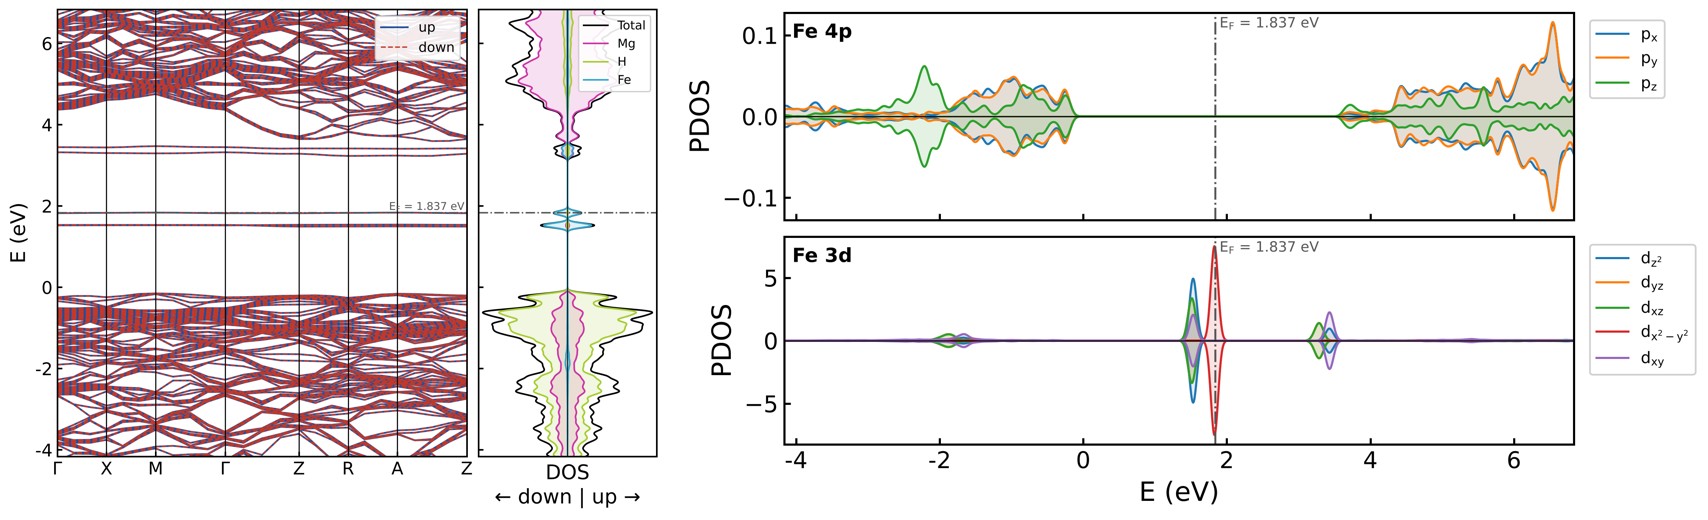
\includegraphics[width=\linewidth]{fermi_python.png}
\caption{MgH$_2$:Fe calculado com o CASTEP e analisado pelo BrUMaRe: bandas com DOS total e projetada (esquerda) e PDOS 4p/3d do Fe (direita), na escala original de energia, com o nível de Fermi marcado.}\label{fig:mgh2}
\end{figure}

\section{Limitações e trabalhos futuros}

O gap e as bordas são avaliados nos pontos $\mathbf k$ do caminho calculado; a DOS obtida de um caminho é apenas ilustrativa. A correção do gap por tesoura não altera a dispersão das bandas nem a posição de níveis de defeito, para as quais são necessários funcionais híbridos ou DFT+U. As energias termodinâmicas não incluem energia de ponto zero. O refinamento das fronteiras de Bader está disponível apenas na linha de comando. Como trabalhos futuros, prevêem-se a função trabalho a partir do potencial eletrostático, as populações de orbitais cristalinos (COHP), dispersões de fônons, propriedades ópticas e o desdobramento de bandas.

\section{Considerações do capítulo}

O BrUMaRe reúne, num programa livre, análises que normalmente exigem várias ferramentas, para cinco programas de estrutura eletrônica, com resultados idênticos no navegador, no aplicativo e na linha de comando. A preservação do nível de Fermi, a exportação de dados em texto, a citação automática e a validação sistemática contra ferramentas consolidadas tornam as análises desta dissertação reprodutíveis e verificáveis. O programa, o tutorial em seis idiomas e a documentação teórica estão disponíveis publicamente.
   e a bibliografia referencias.bib
%  Pacotes usados: amsmath, booktabs, tabularx, graphicx, tikz (positioning, arrows.meta)
% =====================================================================================
\chapter{Desenvolvimento do BrUMaRe: uma ferramenta para o pós-processamento de cálculos de estrutura eletrônica}\label{cap:brumare}

Este capítulo descreve a concepção, a construção e a validação do \textsf{BrUMaRe} (\emph{Brillouin-zone Utilities for Materials Research}), programa livre desenvolvido ao longo desta pesquisa para analisar os resultados dos cálculos de primeiros princípios. O nome une \textbf{Bru}no \textbf{Ma}cedo e \textbf{Re}nata Benedet e é também o acrônimo descrito acima; contém ainda a palavra \emph{bruma}, a névoa que evoca a nuvem eletrônica visualizada pelo programa. A ferramenta nasceu da necessidade prática de analisar, de forma consistente e reprodutível, as estruturas de bandas, as densidades de estados e as densidades de carga do MgH$_2$ com um átomo de Fe substitucional, e foi depois generalizada para qualquer material e para cinco programas de estrutura eletrônica.

\section{Motivação}

O estudo de defeitos em hidretos metálicos por DFT \cite{hohenberg1964,kohn1965} combina vários tipos de análise: estrutura de bandas e densidade de estados (total e projetada), posição dos estados do dopante no gap, distorção local do poliedro de coordenação, energia de formação do defeito, entalpia de formação do hidreto e redistribuição de carga em torno do dopante \cite{sakintuna2007}. Na prática, cada uma dessas análises costuma exigir uma ferramenta diferente: sumo \cite{ganose2018sumo} ou pymatgen \cite{ong2013pymatgen} para bandas, VESTA \cite{momma2011vesta} para densidades, o programa de Bader \cite{henkelman2006} para cargas, além de conversores de formato e scripts próprios. Essa fragmentação traz três problemas:

\begin{enumerate}
\item \textbf{Convenções silenciosas.} A referência de energia de um gráfico de bandas, as unidades de uma grade de densidade ou o fato de o nível de Fermi ter sido recalculado variam de ferramenta para ferramenta, e erros desse tipo passam despercebidos.
\item \textbf{Dificuldade de comparação.} Resultados de programas diferentes (por exemplo, CASTEP e VASP) raramente são comparados num mesmo quadro consistente.
\item \textbf{Reprodutibilidade e crédito.} As figuras são frequentemente publicadas sem os dados numéricos que as originaram e sem a citação de todos os métodos usados.
\end{enumerate}

O \textsf{BrUMaRe} foi construído para resolver esses três pontos, reunindo as análises numa única ferramenta com um modelo de dados comum.

\section{Requisitos}

Os requisitos foram definidos a partir das necessidades desta pesquisa e refinados ao longo do desenvolvimento (Tabela~\ref{tab:requisitos}).

\begin{table}[htbp]\centering\small
\caption{Requisitos do BrUMaRe.}\label{tab:requisitos}
\begin{tabularx}{\linewidth}{@{}lX@{}}\toprule
Requisito & Descrição \\\midrule
R1 · Fermi preservado & O nível de Fermi escrito pelo programa de DFT nunca é recalculado; por padrão as energias são mostradas na escala original, com o $E_\mathrm{F}$ marcado. \\
R2 · Vários programas & Ler CASTEP \cite{clark2005castep}, VASP \cite{kresse1996vasp}, SIESTA \cite{soler2002siesta}, Quantum ESPRESSO \cite{giannozzi2017} e ORCA \cite{neese2020} num modelo de dados único. \\
R3 · Mesmos resultados em todas as interfaces & Navegador (sem instalação), aplicativo de computador (sem internet) e linha de comando (clusters) devem produzir os mesmos números. \\
R4 · Análises completas & Bandas, DOS, PDOS, bandas projetadas, gap, massa efetiva, defeitos, distorção, termodinâmica, densidade, cargas (Voronoi e Bader), diferença de densidade, zona de Brillouin e simetria. \\
R5 · Reprodutibilidade & Toda figura acompanhada de dados em texto (\texttt{.dat}); citação automática dos métodos usados. \\
R6 · Validação & Comparação com ferramentas consolidadas e testes automatizados. \\
R7 · Acesso & Software livre (GPL-3.0), seis idiomas e interface responsiva. \\\bottomrule
\end{tabularx}
\end{table}

\section{Metodologia de desenvolvimento}

O desenvolvimento foi \textbf{iterativo e incremental}: cada versão acrescentou um conjunto de funções, sempre seguido de verificação com arquivos de saída reais. Três práticas guiaram o processo.

\paragraph{Regressão contínua.} Os resultados de um cálculo CASTEP de referência (o MgH$_2$:Fe) foram comparados, a cada mudança, com os da versão anterior; qualquer diferença não intencional era investigada antes de prosseguir.

\paragraph{Validação externa.} As análises foram conferidas contra saídas públicas dos conjuntos de teste do pymatgen, sisl, Quantum ESPRESSO e cclib \cite{oboyle2008cclib}, e contra as próprias ferramentas consolidadas, nos mesmos arquivos (Seção~\ref{sec:validacao}).

\paragraph{Uso declarado de inteligência artificial.} O desenvolvimento contou com o uso extensivo de um modelo de linguagem (Claude, da Anthropic) como assistente de programação, tradução e redação. O escopo científico, a escolha dos métodos e equações, os requisitos e as decisões de projeto foram definidos pelo autor; todo o código gerado com auxílio da IA foi revisado e verificado pelos testes descritos neste capítulo. Essa forma de trabalho mostrou-se produtiva, mas exigiu verificação constante: em mais de uma ocasião, a conferência independente revelou erros (por exemplo, uma explicação física incorreta para a classificação de um isolante como metal por outra ferramenta, e um ponto de alta simetria incorreto no artigo de referência), o que reforça que a responsabilidade pela correção do conteúdo permanece integralmente com o pesquisador.

\section{Arquitetura}

O programa está organizado em três camadas (Figura~\ref{fig:arq}). A \textbf{camada de leitura} converte a saída de cada programa num \textbf{modelo de dados comum}: autovalores em hartree, pontos $\mathbf k$ fracionários, rede em bohr, estruturas em ångström e densidades em e\,Å$^{-3}$. A \textbf{camada de análise} opera apenas sobre esse modelo e atende a três interfaces.

\begin{figure}[htbp]\centering
\resizebox{0.95\linewidth}{!}{\begin{tikzpicture}[node distance=4mm and 5mm, every node/.style={font=\small},
  cx/.style={draw=teal,rounded corners=2pt,fill=teal!6,align=center,minimum height=8mm,inner sep=3pt}]
\node[cx] (c1) {CASTEP}; \node[cx,right=of c1] (c2) {VASP}; \node[cx,right=of c2] (c3) {SIESTA}; \node[cx,right=of c3] (c4) {Quantum ESPRESSO}; \node[cx,right=of c4] (c5) {ORCA};
\node[cx,below=8mm of c3,minimum width=12cm] (m) {Modelo de dados comum (Ha, Å, e\,Å$^{-3}$; $E_\mathrm F$ do programa)};
\node[cx,below=of m,minimum width=12cm] (a) {Análises: DOS/PDOS, gap, $m^*$, defeitos, termodinâmica, densidade, Bader, zona de Brillouin, simetria};
\node[cx,below=8mm of a,xshift=-4cm] (w) {Página web}; \node[cx,below=8mm of a] (d) {Aplicativo (offline)}; \node[cx,below=8mm of a,xshift=4cm] (p) {Linha de comando};
\foreach \c in {c1,c2,c3,c4,c5} \draw[-{Latex[length=2mm]}] (\c.south) -- (m.north -| \c.south);
\draw[-{Latex[length=2mm]}] (m) -- (a); \foreach \f in {w,d,p} \draw[-{Latex[length=2mm]}] (a.south -| \f.north) -- (\f.north);
\end{tikzpicture}}
\caption{Arquitetura do BrUMaRe: leitores específicos, modelo de dados comum, camada de análise e três interfaces com os mesmos resultados.}\label{fig:arq}
\end{figure}

As três interfaces são:
\begin{itemize}
\item \textbf{Página web:} um único arquivo HTML com JavaScript, que roda inteiramente no navegador; os arquivos do usuário nunca são enviados a um servidor.
\item \textbf{Aplicativo de computador:} a mesma página, com todas as bibliotecas incluídas, exibida numa janela própria (pywebview), para Linux, macOS e Windows (instalador \texttt{.exe}).
\item \textbf{Linha de comando:} um único arquivo Python que depende apenas de numpy e matplotlib, adequado a clusters de computação.
\end{itemize}

Uma decisão importante foi o \textbf{registro virtual de arquivos} na versão em Python: os leitores de VASP, SIESTA, QE e ORCA produzem objetos com os nomes que o fluxo do CASTEP espera, de modo que novos programas foram incorporados sem alterar as análises, e a regressão do CASTEP pôde ser mantida idêntica.

A detecção de simetria usa o moyo \cite{moyo}, sucessor do spglib \cite{togo2024spglib}, nas versões idênticas para Python e WebAssembly; a codificação de figuras em JPEG XL usa a libjxl compilada para WebAssembly. Ambas funcionam sem internet.

\section{Métodos implementados}

O documento \emph{Teoria completa do BrUMaRe}, apresentado como apêndice, traz todas as equações. Resumem-se aqui as principais.

\paragraph{Densidade de estados e projeções.} $g_s(E)=\sum_{\mathbf k}w_{\mathbf k}\sum_n\delta_\sigma(E-\varepsilon_{n\mathbf k s})$, com alargamento gaussiano $\delta_\sigma$ e projeções agrupadas por elemento, orbital $l$, camada $(n,l)$, componente $m$ ($t_{2g}/e_g$) ou átomo.

\paragraph{Gap por contagem de elétrons.} Com $N_s$ elétrons no spin $s$, $E_g=\min_{s,\mathbf k}\varepsilon_{N_s+1}-\max_{s,\mathbf k}\varepsilon_{N_s}$. Esse critério é imune a pequenos cruzamentos numéricos do $E_\mathrm F$, que levam ferramentas baseadas apenas em $E_\mathrm F$ a classificar um isolante como metal.

\paragraph{Massa efetiva.} Ajuste $E(k)\simeq c_0+c_1(k-k_0)+c_2(k-k_0)^2$ e $m^*/m_e=\hbar^2/(2m_ec_2)$; o termo linear localiza o extremo verdadeiro entre pontos $\mathbf k$.

\paragraph{Correção do gap.} Tesoura \cite{levine1989} sobre as bandas desocupadas, com $\Delta$ informado, obtido de um gap de referência ou estimado pela relação empírica $E_g^{G_0W_0}=1{,}358E_g^\mathrm{PBE}+0{,}904$\,eV \cite{morales2017}; o $E_\mathrm F$ e as bandas ocupadas não mudam.

\paragraph{Defeitos e termodinâmica.} Casamento por imagem mínima com a estrutura pura, índices de distorção \cite{baur1974,robinson1971,hoppe1979}, energia de formação $E_f=E_\mathrm{def}-E_\mathrm{puro}-\sum_in_i\mu_i$ \cite{freysoldt2014} e temperatura de dessorção $T_d=\Delta H/\Delta S$.

\paragraph{Cargas e diferença de densidade.} Partições de Voronoi \cite{voronoi1908,gellatly1982} e de Bader \cite{bader1990} pelo método sobre a grade \cite{henkelman2006} com refinamento das fronteiras \cite{tang2009bader}; diferença $\Delta\rho$ com carga redistribuída, dipolo e acumulação radial.

\paragraph{Zona de Brillouin e simetria.} A 1.ª zona é a célula de Wigner--Seitz da rede recíproca, construída pelos planos $\mathbf k\cdot\mathbf G=|\mathbf G|^2/2$ sobre base reduzida \cite{lenstra1982}; o grupo espacial é obtido pelo moyo, e as 14 redes de Bravais recebem os pontos e caminhos de \citeonline{setyawan2010}, aceitos apenas se todos os pontos estão na superfície da zona.

\section{Interface, idiomas e acessibilidade}

A interface foi pensada para estudantes e pesquisadores: abas com ícones, tela inicial com os primeiros passos, notificações, atalhos de teclado e editor de gráficos (cores, legendas, estilos). As figuras são exportadas em PNG, JPG, JPEG~XL (sem perdas, idêntico ao PNG), WEBP e SVG. Interface, tutorial e ajuda estão disponíveis em português, inglês, espanhol, francês, italiano e latim; a página foi verificada em larguras de 320\,px a 4K, sem rolagem horizontal.

\section{Distribuição e licença}

O programa é distribuído sob a licença GPL-3.0-or-later, como página web, como pacote Python (\texttt{pip install brumare}) e como instalador para Windows, gerado automaticamente por integração contínua. Cada sessão gera um arquivo BibTeX com o próprio BrUMaRe, os programas de DFT cujas saídas foram usadas e os métodos efetivamente aplicados, o que facilita a citação correta.

\section{Verificação e validação}\label{sec:validacao}

\paragraph{Sistemas de referência.} A Tabela~\ref{tab:val} reúne resultados obtidos com saídas reais.

\begin{table}[htbp]\centering\small
\caption{Validação com saídas reais (gaps de Kohn--Sham de cada funcional).}\label{tab:val}
\begin{tabularx}{\linewidth}{@{}llX@{}}\toprule
Programa & Sistema & Resultado \\\midrule
CASTEP & MgH$_2$:Fe (162 átomos) & gap 1,394\,eV (M$\to$R); Fe--H 1,649--1,653\,Å \\
VASP & Si (PBE) & gap 0,614\,eV; $m^*_e=0{,}94\,m_e$ (experimental 0,92) \\
VASP & Fe$_2$O$_3$ (LDA+U) & 20\,$\mu_\mathrm B$ (quatro Fe$^{3+}$ de spin alto) \\
SIESTA & SrTiO$_3$ e Bi$_2$Se$_3$ & gaps idênticos aos do sisl \\
Quantum ESPRESSO & Si & gap 1,32\,eV na malha do teste \\
ORCA & divinilbenzeno & gap HOMO--LUMO 5,18\,eV, igual ao cclib \\\bottomrule
\end{tabularx}
\end{table}

\paragraph{Comparação com ferramentas consolidadas.} Nos mesmos arquivos, gaps, bordas, níveis de Fermi, contagens de elétrons e energias de orbitais coincidem com pymatgen, sumo, sisl e cclib até a precisão impressa. Duas diferenças são de método e favorecem a abordagem adotada: (i) no MgH$_2$:Fe, o topo da banda ocupada fica 0,04--0,17\,meV acima do $E_\mathrm F$ escrito pelo CASTEP, e o sumo classifica o sistema como metal (gap nulo), enquanto a contagem de elétrons dá 1,394\,eV; (ii) no Si, o mínimo da banda de condução fica entre dois pontos $\mathbf k$, e uma parábola ancorada no ponto amostrado dá 0,68 ou 1,54\,$m_e$, enquanto o ajuste com termo linear dá 0,94\,$m_e$. As cargas de Bader refinadas coincidem com as do pybader em $8\times10^{-4}$\,e por átomo, em média.

\paragraph{Simetria e zona de Brillouin.} Os grupos espaciais dos 51 materiais da biblioteca e de 22 estruturas de teste são recuperados nas duas implementações; para 18 estruturas que cobrem as 14 redes de Bravais, os módulos $|\mathbf k|$ dos pontos de alta simetria coincidem com a implementação independente do pymatgen até $10^{-8}$\,Å$^{-1}$, e a página e o Python dão pontos idênticos. A verificação revelou que o ponto $F_3$ do caso MCLC1 no artigo original não está na superfície da zona; ele não faz parte do caminho e foi omitido.

\paragraph{Testes automatizados.} Um conjunto de 80 testes (\texttt{pytest}) com saídas reais é executado automaticamente a cada alteração do código, em duas versões do Python.

\section{Aplicação ao MgH\texorpdfstring{$_2$}{2}:Fe}

Para a supercélula $3\times3\times3$ do MgH$_2$ rutilo com um Fe substitucional (162 átomos), o BrUMaRe lê $E_\mathrm F^\uparrow=0{,}067501$\,Ha e $E_\mathrm F^\downarrow=0{,}067499$\,Ha e encontra um gap total de 1,394\,eV, indireto entre M e R, com estados $d$ do Fe dentro do gap do hospedeiro (Figura~\ref{fig:mgh2}). O octaedro FeH$_6$ é quase regular ($\langle\lambda\rangle=1{,}0004$, $\sigma^2=1{,}5$\,graus$^2$), com ligações Fe--H 15,4\,\% mais curtas que as Mg--H do material puro. A análise de simetria mostra que a supercélula relaxada pertence ao grupo $Cmmm$ (ortorrômbico de base centrada), resultado da combinação do defeito com a relaxação, e o caminho de bandas correspondente é gerado automaticamente.

\begin{figure}[htbp]\centering
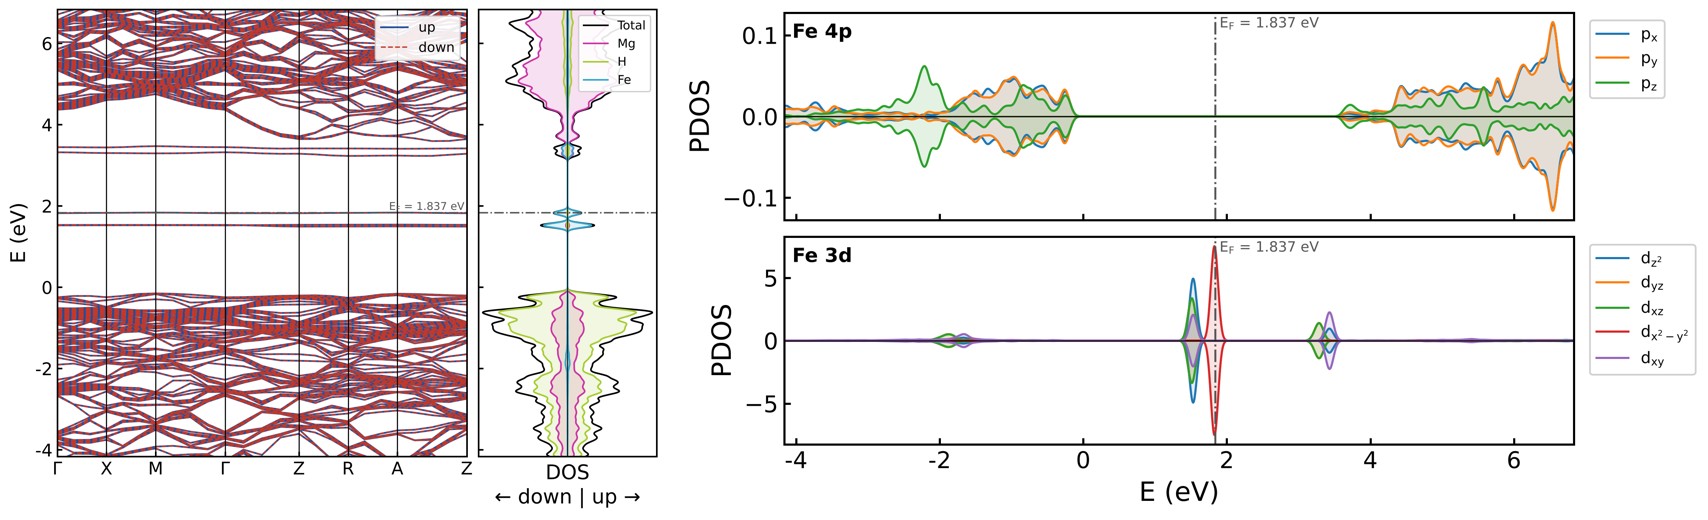
\includegraphics[width=\linewidth]{fermi_python.png}
\caption{MgH$_2$:Fe calculado com o CASTEP e analisado pelo BrUMaRe: bandas com DOS total e projetada (esquerda) e PDOS 4p/3d do Fe (direita), na escala original de energia, com o nível de Fermi marcado.}\label{fig:mgh2}
\end{figure}

\section{Limitações e trabalhos futuros}

O gap e as bordas são avaliados nos pontos $\mathbf k$ do caminho calculado; a DOS obtida de um caminho é apenas ilustrativa. A correção do gap por tesoura não altera a dispersão das bandas nem a posição de níveis de defeito, para as quais são necessários funcionais híbridos ou DFT+U. As energias termodinâmicas não incluem energia de ponto zero. O refinamento das fronteiras de Bader está disponível apenas na linha de comando. Como trabalhos futuros, prevêem-se a função trabalho a partir do potencial eletrostático, as populações de orbitais cristalinos (COHP), dispersões de fônons, propriedades ópticas e o desdobramento de bandas.

\section{Considerações do capítulo}

O BrUMaRe reúne, num programa livre, análises que normalmente exigem várias ferramentas, para cinco programas de estrutura eletrônica, com resultados idênticos no navegador, no aplicativo e na linha de comando. A preservação do nível de Fermi, a exportação de dados em texto, a citação automática e a validação sistemática contra ferramentas consolidadas tornam as análises desta dissertação reprodutíveis e verificáveis. O programa, o tutorial em seis idiomas e a documentação teórica estão disponíveis publicamente.
   e a bibliografia referencias.bib
%  Pacotes usados: amsmath, booktabs, tabularx, graphicx, tikz (positioning, arrows.meta)
% =====================================================================================
\chapter{Desenvolvimento do BrUMaRe: uma ferramenta para o pós-processamento de cálculos de estrutura eletrônica}\label{cap:brumare}

Este capítulo descreve a concepção, a construção e a validação do \textsf{BrUMaRe} (\emph{Brillouin-zone Utilities for Materials Research}), programa livre desenvolvido ao longo desta pesquisa para analisar os resultados dos cálculos de primeiros princípios. O nome une \textbf{Bru}no \textbf{Ma}cedo e \textbf{Re}nata Benedet e é também o acrônimo descrito acima; contém ainda a palavra \emph{bruma}, a névoa que evoca a nuvem eletrônica visualizada pelo programa. A ferramenta nasceu da necessidade prática de analisar, de forma consistente e reprodutível, as estruturas de bandas, as densidades de estados e as densidades de carga do MgH$_2$ com um átomo de Fe substitucional, e foi depois generalizada para qualquer material e para cinco programas de estrutura eletrônica.

\section{Motivação}

O estudo de defeitos em hidretos metálicos por DFT \cite{hohenberg1964,kohn1965} combina vários tipos de análise: estrutura de bandas e densidade de estados (total e projetada), posição dos estados do dopante no gap, distorção local do poliedro de coordenação, energia de formação do defeito, entalpia de formação do hidreto e redistribuição de carga em torno do dopante \cite{sakintuna2007}. Na prática, cada uma dessas análises costuma exigir uma ferramenta diferente: sumo \cite{ganose2018sumo} ou pymatgen \cite{ong2013pymatgen} para bandas, VESTA \cite{momma2011vesta} para densidades, o programa de Bader \cite{henkelman2006} para cargas, além de conversores de formato e scripts próprios. Essa fragmentação traz três problemas:

\begin{enumerate}
\item \textbf{Convenções silenciosas.} A referência de energia de um gráfico de bandas, as unidades de uma grade de densidade ou o fato de o nível de Fermi ter sido recalculado variam de ferramenta para ferramenta, e erros desse tipo passam despercebidos.
\item \textbf{Dificuldade de comparação.} Resultados de programas diferentes (por exemplo, CASTEP e VASP) raramente são comparados num mesmo quadro consistente.
\item \textbf{Reprodutibilidade e crédito.} As figuras são frequentemente publicadas sem os dados numéricos que as originaram e sem a citação de todos os métodos usados.
\end{enumerate}

O \textsf{BrUMaRe} foi construído para resolver esses três pontos, reunindo as análises numa única ferramenta com um modelo de dados comum.

\section{Requisitos}

Os requisitos foram definidos a partir das necessidades desta pesquisa e refinados ao longo do desenvolvimento (Tabela~\ref{tab:requisitos}).

\begin{table}[htbp]\centering\small
\caption{Requisitos do BrUMaRe.}\label{tab:requisitos}
\begin{tabularx}{\linewidth}{@{}lX@{}}\toprule
Requisito & Descrição \\\midrule
R1 · Fermi preservado & O nível de Fermi escrito pelo programa de DFT nunca é recalculado; por padrão as energias são mostradas na escala original, com o $E_\mathrm{F}$ marcado. \\
R2 · Vários programas & Ler CASTEP \cite{clark2005castep}, VASP \cite{kresse1996vasp}, SIESTA \cite{soler2002siesta}, Quantum ESPRESSO \cite{giannozzi2017} e ORCA \cite{neese2020} num modelo de dados único. \\
R3 · Mesmos resultados em todas as interfaces & Navegador (sem instalação), aplicativo de computador (sem internet) e linha de comando (clusters) devem produzir os mesmos números. \\
R4 · Análises completas & Bandas, DOS, PDOS, bandas projetadas, gap, massa efetiva, defeitos, distorção, termodinâmica, densidade, cargas (Voronoi e Bader), diferença de densidade, zona de Brillouin e simetria. \\
R5 · Reprodutibilidade & Toda figura acompanhada de dados em texto (\texttt{.dat}); citação automática dos métodos usados. \\
R6 · Validação & Comparação com ferramentas consolidadas e testes automatizados. \\
R7 · Acesso & Software livre (GPL-3.0), seis idiomas e interface responsiva. \\\bottomrule
\end{tabularx}
\end{table}

\section{Metodologia de desenvolvimento}

O desenvolvimento foi \textbf{iterativo e incremental}: cada versão acrescentou um conjunto de funções, sempre seguido de verificação com arquivos de saída reais. Três práticas guiaram o processo.

\paragraph{Regressão contínua.} Os resultados de um cálculo CASTEP de referência (o MgH$_2$:Fe) foram comparados, a cada mudança, com os da versão anterior; qualquer diferença não intencional era investigada antes de prosseguir.

\paragraph{Validação externa.} As análises foram conferidas contra saídas públicas dos conjuntos de teste do pymatgen, sisl, Quantum ESPRESSO e cclib \cite{oboyle2008cclib}, e contra as próprias ferramentas consolidadas, nos mesmos arquivos (Seção~\ref{sec:validacao}).

\paragraph{Uso declarado de inteligência artificial.} O desenvolvimento contou com o uso extensivo de um modelo de linguagem (Claude, da Anthropic) como assistente de programação, tradução e redação. O escopo científico, a escolha dos métodos e equações, os requisitos e as decisões de projeto foram definidos pelo autor; todo o código gerado com auxílio da IA foi revisado e verificado pelos testes descritos neste capítulo. Essa forma de trabalho mostrou-se produtiva, mas exigiu verificação constante: em mais de uma ocasião, a conferência independente revelou erros (por exemplo, uma explicação física incorreta para a classificação de um isolante como metal por outra ferramenta, e um ponto de alta simetria incorreto no artigo de referência), o que reforça que a responsabilidade pela correção do conteúdo permanece integralmente com o pesquisador.

\section{Arquitetura}

O programa está organizado em três camadas (Figura~\ref{fig:arq}). A \textbf{camada de leitura} converte a saída de cada programa num \textbf{modelo de dados comum}: autovalores em hartree, pontos $\mathbf k$ fracionários, rede em bohr, estruturas em ångström e densidades em e\,Å$^{-3}$. A \textbf{camada de análise} opera apenas sobre esse modelo e atende a três interfaces.

\begin{figure}[htbp]\centering
\resizebox{0.95\linewidth}{!}{\begin{tikzpicture}[node distance=4mm and 5mm, every node/.style={font=\small},
  cx/.style={draw=teal,rounded corners=2pt,fill=teal!6,align=center,minimum height=8mm,inner sep=3pt}]
\node[cx] (c1) {CASTEP}; \node[cx,right=of c1] (c2) {VASP}; \node[cx,right=of c2] (c3) {SIESTA}; \node[cx,right=of c3] (c4) {Quantum ESPRESSO}; \node[cx,right=of c4] (c5) {ORCA};
\node[cx,below=8mm of c3,minimum width=12cm] (m) {Modelo de dados comum (Ha, Å, e\,Å$^{-3}$; $E_\mathrm F$ do programa)};
\node[cx,below=of m,minimum width=12cm] (a) {Análises: DOS/PDOS, gap, $m^*$, defeitos, termodinâmica, densidade, Bader, zona de Brillouin, simetria};
\node[cx,below=8mm of a,xshift=-4cm] (w) {Página web}; \node[cx,below=8mm of a] (d) {Aplicativo (offline)}; \node[cx,below=8mm of a,xshift=4cm] (p) {Linha de comando};
\foreach \c in {c1,c2,c3,c4,c5} \draw[-{Latex[length=2mm]}] (\c.south) -- (m.north -| \c.south);
\draw[-{Latex[length=2mm]}] (m) -- (a); \foreach \f in {w,d,p} \draw[-{Latex[length=2mm]}] (a.south -| \f.north) -- (\f.north);
\end{tikzpicture}}
\caption{Arquitetura do BrUMaRe: leitores específicos, modelo de dados comum, camada de análise e três interfaces com os mesmos resultados.}\label{fig:arq}
\end{figure}

As três interfaces são:
\begin{itemize}
\item \textbf{Página web:} um único arquivo HTML com JavaScript, que roda inteiramente no navegador; os arquivos do usuário nunca são enviados a um servidor.
\item \textbf{Aplicativo de computador:} a mesma página, com todas as bibliotecas incluídas, exibida numa janela própria (pywebview), para Linux, macOS e Windows (instalador \texttt{.exe}).
\item \textbf{Linha de comando:} um único arquivo Python que depende apenas de numpy e matplotlib, adequado a clusters de computação.
\end{itemize}

Uma decisão importante foi o \textbf{registro virtual de arquivos} na versão em Python: os leitores de VASP, SIESTA, QE e ORCA produzem objetos com os nomes que o fluxo do CASTEP espera, de modo que novos programas foram incorporados sem alterar as análises, e a regressão do CASTEP pôde ser mantida idêntica.

A detecção de simetria usa o moyo \cite{moyo}, sucessor do spglib \cite{togo2024spglib}, nas versões idênticas para Python e WebAssembly; a codificação de figuras em JPEG XL usa a libjxl compilada para WebAssembly. Ambas funcionam sem internet.

\section{Métodos implementados}

O documento \emph{Teoria completa do BrUMaRe}, apresentado como apêndice, traz todas as equações. Resumem-se aqui as principais.

\paragraph{Densidade de estados e projeções.} $g_s(E)=\sum_{\mathbf k}w_{\mathbf k}\sum_n\delta_\sigma(E-\varepsilon_{n\mathbf k s})$, com alargamento gaussiano $\delta_\sigma$ e projeções agrupadas por elemento, orbital $l$, camada $(n,l)$, componente $m$ ($t_{2g}/e_g$) ou átomo.

\paragraph{Gap por contagem de elétrons.} Com $N_s$ elétrons no spin $s$, $E_g=\min_{s,\mathbf k}\varepsilon_{N_s+1}-\max_{s,\mathbf k}\varepsilon_{N_s}$. Esse critério é imune a pequenos cruzamentos numéricos do $E_\mathrm F$, que levam ferramentas baseadas apenas em $E_\mathrm F$ a classificar um isolante como metal.

\paragraph{Massa efetiva.} Ajuste $E(k)\simeq c_0+c_1(k-k_0)+c_2(k-k_0)^2$ e $m^*/m_e=\hbar^2/(2m_ec_2)$; o termo linear localiza o extremo verdadeiro entre pontos $\mathbf k$.

\paragraph{Correção do gap.} Tesoura \cite{levine1989} sobre as bandas desocupadas, com $\Delta$ informado, obtido de um gap de referência ou estimado pela relação empírica $E_g^{G_0W_0}=1{,}358E_g^\mathrm{PBE}+0{,}904$\,eV \cite{morales2017}; o $E_\mathrm F$ e as bandas ocupadas não mudam.

\paragraph{Defeitos e termodinâmica.} Casamento por imagem mínima com a estrutura pura, índices de distorção \cite{baur1974,robinson1971,hoppe1979}, energia de formação $E_f=E_\mathrm{def}-E_\mathrm{puro}-\sum_in_i\mu_i$ \cite{freysoldt2014} e temperatura de dessorção $T_d=\Delta H/\Delta S$.

\paragraph{Cargas e diferença de densidade.} Partições de Voronoi \cite{voronoi1908,gellatly1982} e de Bader \cite{bader1990} pelo método sobre a grade \cite{henkelman2006} com refinamento das fronteiras \cite{tang2009bader}; diferença $\Delta\rho$ com carga redistribuída, dipolo e acumulação radial.

\paragraph{Zona de Brillouin e simetria.} A 1.ª zona é a célula de Wigner--Seitz da rede recíproca, construída pelos planos $\mathbf k\cdot\mathbf G=|\mathbf G|^2/2$ sobre base reduzida \cite{lenstra1982}; o grupo espacial é obtido pelo moyo, e as 14 redes de Bravais recebem os pontos e caminhos de \citeonline{setyawan2010}, aceitos apenas se todos os pontos estão na superfície da zona.

\section{Interface, idiomas e acessibilidade}

A interface foi pensada para estudantes e pesquisadores: abas com ícones, tela inicial com os primeiros passos, notificações, atalhos de teclado e editor de gráficos (cores, legendas, estilos). As figuras são exportadas em PNG, JPG, JPEG~XL (sem perdas, idêntico ao PNG), WEBP e SVG. Interface, tutorial e ajuda estão disponíveis em português, inglês, espanhol, francês, italiano e latim; a página foi verificada em larguras de 320\,px a 4K, sem rolagem horizontal.

\section{Distribuição e licença}

O programa é distribuído sob a licença GPL-3.0-or-later, como página web, como pacote Python (\texttt{pip install brumare}) e como instalador para Windows, gerado automaticamente por integração contínua. Cada sessão gera um arquivo BibTeX com o próprio BrUMaRe, os programas de DFT cujas saídas foram usadas e os métodos efetivamente aplicados, o que facilita a citação correta.

\section{Verificação e validação}\label{sec:validacao}

\paragraph{Sistemas de referência.} A Tabela~\ref{tab:val} reúne resultados obtidos com saídas reais.

\begin{table}[htbp]\centering\small
\caption{Validação com saídas reais (gaps de Kohn--Sham de cada funcional).}\label{tab:val}
\begin{tabularx}{\linewidth}{@{}llX@{}}\toprule
Programa & Sistema & Resultado \\\midrule
CASTEP & MgH$_2$:Fe (162 átomos) & gap 1,394\,eV (M$\to$R); Fe--H 1,649--1,653\,Å \\
VASP & Si (PBE) & gap 0,614\,eV; $m^*_e=0{,}94\,m_e$ (experimental 0,92) \\
VASP & Fe$_2$O$_3$ (LDA+U) & 20\,$\mu_\mathrm B$ (quatro Fe$^{3+}$ de spin alto) \\
SIESTA & SrTiO$_3$ e Bi$_2$Se$_3$ & gaps idênticos aos do sisl \\
Quantum ESPRESSO & Si & gap 1,32\,eV na malha do teste \\
ORCA & divinilbenzeno & gap HOMO--LUMO 5,18\,eV, igual ao cclib \\\bottomrule
\end{tabularx}
\end{table}

\paragraph{Comparação com ferramentas consolidadas.} Nos mesmos arquivos, gaps, bordas, níveis de Fermi, contagens de elétrons e energias de orbitais coincidem com pymatgen, sumo, sisl e cclib até a precisão impressa. Duas diferenças são de método e favorecem a abordagem adotada: (i) no MgH$_2$:Fe, o topo da banda ocupada fica 0,04--0,17\,meV acima do $E_\mathrm F$ escrito pelo CASTEP, e o sumo classifica o sistema como metal (gap nulo), enquanto a contagem de elétrons dá 1,394\,eV; (ii) no Si, o mínimo da banda de condução fica entre dois pontos $\mathbf k$, e uma parábola ancorada no ponto amostrado dá 0,68 ou 1,54\,$m_e$, enquanto o ajuste com termo linear dá 0,94\,$m_e$. As cargas de Bader refinadas coincidem com as do pybader em $8\times10^{-4}$\,e por átomo, em média.

\paragraph{Simetria e zona de Brillouin.} Os grupos espaciais dos 51 materiais da biblioteca e de 22 estruturas de teste são recuperados nas duas implementações; para 18 estruturas que cobrem as 14 redes de Bravais, os módulos $|\mathbf k|$ dos pontos de alta simetria coincidem com a implementação independente do pymatgen até $10^{-8}$\,Å$^{-1}$, e a página e o Python dão pontos idênticos. A verificação revelou que o ponto $F_3$ do caso MCLC1 no artigo original não está na superfície da zona; ele não faz parte do caminho e foi omitido.

\paragraph{Testes automatizados.} Um conjunto de 80 testes (\texttt{pytest}) com saídas reais é executado automaticamente a cada alteração do código, em duas versões do Python.

\section{Aplicação ao MgH\texorpdfstring{$_2$}{2}:Fe}

Para a supercélula $3\times3\times3$ do MgH$_2$ rutilo com um Fe substitucional (162 átomos), o BrUMaRe lê $E_\mathrm F^\uparrow=0{,}067501$\,Ha e $E_\mathrm F^\downarrow=0{,}067499$\,Ha e encontra um gap total de 1,394\,eV, indireto entre M e R, com estados $d$ do Fe dentro do gap do hospedeiro (Figura~\ref{fig:mgh2}). O octaedro FeH$_6$ é quase regular ($\langle\lambda\rangle=1{,}0004$, $\sigma^2=1{,}5$\,graus$^2$), com ligações Fe--H 15,4\,\% mais curtas que as Mg--H do material puro. A análise de simetria mostra que a supercélula relaxada pertence ao grupo $Cmmm$ (ortorrômbico de base centrada), resultado da combinação do defeito com a relaxação, e o caminho de bandas correspondente é gerado automaticamente.

\begin{figure}[htbp]\centering
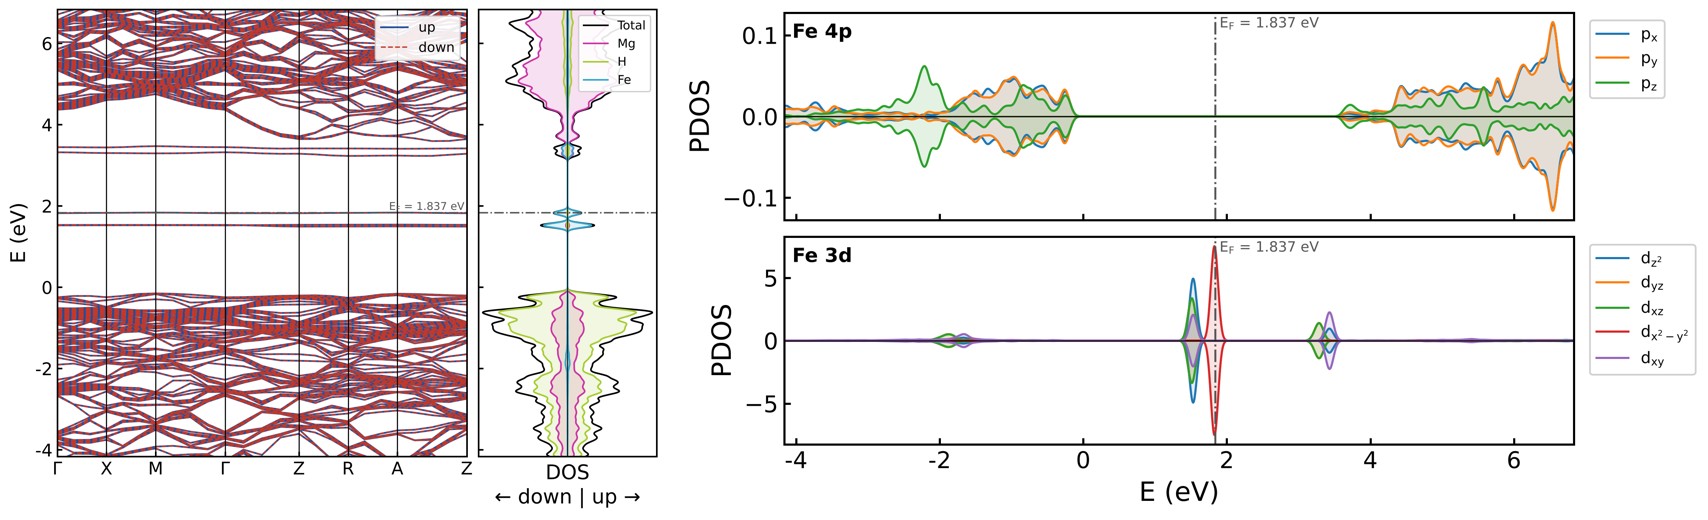
\includegraphics[width=\linewidth]{fermi_python.png}
\caption{MgH$_2$:Fe calculado com o CASTEP e analisado pelo BrUMaRe: bandas com DOS total e projetada (esquerda) e PDOS 4p/3d do Fe (direita), na escala original de energia, com o nível de Fermi marcado.}\label{fig:mgh2}
\end{figure}

\section{Limitações e trabalhos futuros}

O gap e as bordas são avaliados nos pontos $\mathbf k$ do caminho calculado; a DOS obtida de um caminho é apenas ilustrativa. A correção do gap por tesoura não altera a dispersão das bandas nem a posição de níveis de defeito, para as quais são necessários funcionais híbridos ou DFT+U. As energias termodinâmicas não incluem energia de ponto zero. O refinamento das fronteiras de Bader está disponível apenas na linha de comando. Como trabalhos futuros, prevêem-se a função trabalho a partir do potencial eletrostático, as populações de orbitais cristalinos (COHP), dispersões de fônons, propriedades ópticas e o desdobramento de bandas.

\section{Considerações do capítulo}

O BrUMaRe reúne, num programa livre, análises que normalmente exigem várias ferramentas, para cinco programas de estrutura eletrônica, com resultados idênticos no navegador, no aplicativo e na linha de comando. A preservação do nível de Fermi, a exportação de dados em texto, a citação automática e a validação sistemática contra ferramentas consolidadas tornam as análises desta dissertação reprodutíveis e verificáveis. O programa, o tutorial em seis idiomas e a documentação teórica estão disponíveis publicamente.
   e a bibliografia referencias.bib
%  Pacotes usados: amsmath, booktabs, tabularx, graphicx, tikz (positioning, arrows.meta)
% =====================================================================================
\chapter{Desenvolvimento do BrUMaRe: uma ferramenta para o pós-processamento de cálculos de estrutura eletrônica}\label{cap:brumare}

Este capítulo descreve a concepção, a construção e a validação do \textsf{BrUMaRe} (\emph{Brillouin-zone Utilities for Materials Research}), programa livre desenvolvido ao longo desta pesquisa para analisar os resultados dos cálculos de primeiros princípios. O nome une \textbf{Bru}no \textbf{Ma}cedo e \textbf{Re}nata Benedet e é também o acrônimo descrito acima; contém ainda a palavra \emph{bruma}, a névoa que evoca a nuvem eletrônica visualizada pelo programa. A ferramenta nasceu da necessidade prática de analisar, de forma consistente e reprodutível, as estruturas de bandas, as densidades de estados e as densidades de carga do MgH$_2$ com um átomo de Fe substitucional, e foi depois generalizada para qualquer material e para cinco programas de estrutura eletrônica.

\section{Motivação}

O estudo de defeitos em hidretos metálicos por DFT \cite{hohenberg1964,kohn1965} combina vários tipos de análise: estrutura de bandas e densidade de estados (total e projetada), posição dos estados do dopante no gap, distorção local do poliedro de coordenação, energia de formação do defeito, entalpia de formação do hidreto e redistribuição de carga em torno do dopante \cite{sakintuna2007}. Na prática, cada uma dessas análises costuma exigir uma ferramenta diferente: sumo \cite{ganose2018sumo} ou pymatgen \cite{ong2013pymatgen} para bandas, VESTA \cite{momma2011vesta} para densidades, o programa de Bader \cite{henkelman2006} para cargas, além de conversores de formato e scripts próprios. Essa fragmentação traz três problemas:

\begin{enumerate}
\item \textbf{Convenções silenciosas.} A referência de energia de um gráfico de bandas, as unidades de uma grade de densidade ou o fato de o nível de Fermi ter sido recalculado variam de ferramenta para ferramenta, e erros desse tipo passam despercebidos.
\item \textbf{Dificuldade de comparação.} Resultados de programas diferentes (por exemplo, CASTEP e VASP) raramente são comparados num mesmo quadro consistente.
\item \textbf{Reprodutibilidade e crédito.} As figuras são frequentemente publicadas sem os dados numéricos que as originaram e sem a citação de todos os métodos usados.
\end{enumerate}

O \textsf{BrUMaRe} foi construído para resolver esses três pontos, reunindo as análises numa única ferramenta com um modelo de dados comum.

\section{Requisitos}

Os requisitos foram definidos a partir das necessidades desta pesquisa e refinados ao longo do desenvolvimento (Tabela~\ref{tab:requisitos}).

\begin{table}[htbp]\centering\small
\caption{Requisitos do BrUMaRe.}\label{tab:requisitos}
\begin{tabularx}{\linewidth}{@{}lX@{}}\toprule
Requisito & Descrição \\\midrule
R1 · Fermi preservado & O nível de Fermi escrito pelo programa de DFT nunca é recalculado; por padrão as energias são mostradas na escala original, com o $E_\mathrm{F}$ marcado. \\
R2 · Vários programas & Ler CASTEP \cite{clark2005castep}, VASP \cite{kresse1996vasp}, SIESTA \cite{soler2002siesta}, Quantum ESPRESSO \cite{giannozzi2017} e ORCA \cite{neese2020} num modelo de dados único. \\
R3 · Mesmos resultados em todas as interfaces & Navegador (sem instalação), aplicativo de computador (sem internet) e linha de comando (clusters) devem produzir os mesmos números. \\
R4 · Análises completas & Bandas, DOS, PDOS, bandas projetadas, gap, massa efetiva, defeitos, distorção, termodinâmica, densidade, cargas (Voronoi e Bader), diferença de densidade, zona de Brillouin e simetria. \\
R5 · Reprodutibilidade & Toda figura acompanhada de dados em texto (\texttt{.dat}); citação automática dos métodos usados. \\
R6 · Validação & Comparação com ferramentas consolidadas e testes automatizados. \\
R7 · Acesso & Software livre (GPL-3.0), seis idiomas e interface responsiva. \\\bottomrule
\end{tabularx}
\end{table}

\section{Metodologia de desenvolvimento}

O desenvolvimento foi \textbf{iterativo e incremental}: cada versão acrescentou um conjunto de funções, sempre seguido de verificação com arquivos de saída reais. Três práticas guiaram o processo.

\paragraph{Regressão contínua.} Os resultados de um cálculo CASTEP de referência (o MgH$_2$:Fe) foram comparados, a cada mudança, com os da versão anterior; qualquer diferença não intencional era investigada antes de prosseguir.

\paragraph{Validação externa.} As análises foram conferidas contra saídas públicas dos conjuntos de teste do pymatgen, sisl, Quantum ESPRESSO e cclib \cite{oboyle2008cclib}, e contra as próprias ferramentas consolidadas, nos mesmos arquivos (Seção~\ref{sec:validacao}).

\paragraph{Uso declarado de inteligência artificial.} O desenvolvimento contou com o uso extensivo de um modelo de linguagem (Claude, da Anthropic) como assistente de programação, tradução e redação. O escopo científico, a escolha dos métodos e equações, os requisitos e as decisões de projeto foram definidos pelo autor; todo o código gerado com auxílio da IA foi revisado e verificado pelos testes descritos neste capítulo. Essa forma de trabalho mostrou-se produtiva, mas exigiu verificação constante: em mais de uma ocasião, a conferência independente revelou erros (por exemplo, uma explicação física incorreta para a classificação de um isolante como metal por outra ferramenta, e um ponto de alta simetria incorreto no artigo de referência), o que reforça que a responsabilidade pela correção do conteúdo permanece integralmente com o pesquisador.

\section{Arquitetura}

O programa está organizado em três camadas (Figura~\ref{fig:arq}). A \textbf{camada de leitura} converte a saída de cada programa num \textbf{modelo de dados comum}: autovalores em hartree, pontos $\mathbf k$ fracionários, rede em bohr, estruturas em ångström e densidades em e\,Å$^{-3}$. A \textbf{camada de análise} opera apenas sobre esse modelo e atende a três interfaces.

\begin{figure}[htbp]\centering
\resizebox{0.95\linewidth}{!}{\begin{tikzpicture}[node distance=4mm and 5mm, every node/.style={font=\small},
  cx/.style={draw=teal,rounded corners=2pt,fill=teal!6,align=center,minimum height=8mm,inner sep=3pt}]
\node[cx] (c1) {CASTEP}; \node[cx,right=of c1] (c2) {VASP}; \node[cx,right=of c2] (c3) {SIESTA}; \node[cx,right=of c3] (c4) {Quantum ESPRESSO}; \node[cx,right=of c4] (c5) {ORCA};
\node[cx,below=8mm of c3,minimum width=12cm] (m) {Modelo de dados comum (Ha, Å, e\,Å$^{-3}$; $E_\mathrm F$ do programa)};
\node[cx,below=of m,minimum width=12cm] (a) {Análises: DOS/PDOS, gap, $m^*$, defeitos, termodinâmica, densidade, Bader, zona de Brillouin, simetria};
\node[cx,below=8mm of a,xshift=-4cm] (w) {Página web}; \node[cx,below=8mm of a] (d) {Aplicativo (offline)}; \node[cx,below=8mm of a,xshift=4cm] (p) {Linha de comando};
\foreach \c in {c1,c2,c3,c4,c5} \draw[-{Latex[length=2mm]}] (\c.south) -- (m.north -| \c.south);
\draw[-{Latex[length=2mm]}] (m) -- (a); \foreach \f in {w,d,p} \draw[-{Latex[length=2mm]}] (a.south -| \f.north) -- (\f.north);
\end{tikzpicture}}
\caption{Arquitetura do BrUMaRe: leitores específicos, modelo de dados comum, camada de análise e três interfaces com os mesmos resultados.}\label{fig:arq}
\end{figure}

As três interfaces são:
\begin{itemize}
\item \textbf{Página web:} um único arquivo HTML com JavaScript, que roda inteiramente no navegador; os arquivos do usuário nunca são enviados a um servidor.
\item \textbf{Aplicativo de computador:} a mesma página, com todas as bibliotecas incluídas, exibida numa janela própria (pywebview), para Linux, macOS e Windows (instalador \texttt{.exe}).
\item \textbf{Linha de comando:} um único arquivo Python que depende apenas de numpy e matplotlib, adequado a clusters de computação.
\end{itemize}

Uma decisão importante foi o \textbf{registro virtual de arquivos} na versão em Python: os leitores de VASP, SIESTA, QE e ORCA produzem objetos com os nomes que o fluxo do CASTEP espera, de modo que novos programas foram incorporados sem alterar as análises, e a regressão do CASTEP pôde ser mantida idêntica.

A detecção de simetria usa o moyo \cite{moyo}, sucessor do spglib \cite{togo2024spglib}, nas versões idênticas para Python e WebAssembly; a codificação de figuras em JPEG XL usa a libjxl compilada para WebAssembly. Ambas funcionam sem internet.

\section{Métodos implementados}

O documento \emph{Teoria completa do BrUMaRe}, apresentado como apêndice, traz todas as equações. Resumem-se aqui as principais.

\paragraph{Densidade de estados e projeções.} $g_s(E)=\sum_{\mathbf k}w_{\mathbf k}\sum_n\delta_\sigma(E-\varepsilon_{n\mathbf k s})$, com alargamento gaussiano $\delta_\sigma$ e projeções agrupadas por elemento, orbital $l$, camada $(n,l)$, componente $m$ ($t_{2g}/e_g$) ou átomo.

\paragraph{Gap por contagem de elétrons.} Com $N_s$ elétrons no spin $s$, $E_g=\min_{s,\mathbf k}\varepsilon_{N_s+1}-\max_{s,\mathbf k}\varepsilon_{N_s}$. Esse critério é imune a pequenos cruzamentos numéricos do $E_\mathrm F$, que levam ferramentas baseadas apenas em $E_\mathrm F$ a classificar um isolante como metal.

\paragraph{Massa efetiva.} Ajuste $E(k)\simeq c_0+c_1(k-k_0)+c_2(k-k_0)^2$ e $m^*/m_e=\hbar^2/(2m_ec_2)$; o termo linear localiza o extremo verdadeiro entre pontos $\mathbf k$.

\paragraph{Correção do gap.} Tesoura \cite{levine1989} sobre as bandas desocupadas, com $\Delta$ informado, obtido de um gap de referência ou estimado pela relação empírica $E_g^{G_0W_0}=1{,}358E_g^\mathrm{PBE}+0{,}904$\,eV \cite{morales2017}; o $E_\mathrm F$ e as bandas ocupadas não mudam.

\paragraph{Defeitos e termodinâmica.} Casamento por imagem mínima com a estrutura pura, índices de distorção \cite{baur1974,robinson1971,hoppe1979}, energia de formação $E_f=E_\mathrm{def}-E_\mathrm{puro}-\sum_in_i\mu_i$ \cite{freysoldt2014} e temperatura de dessorção $T_d=\Delta H/\Delta S$.

\paragraph{Cargas e diferença de densidade.} Partições de Voronoi \cite{voronoi1908,gellatly1982} e de Bader \cite{bader1990} pelo método sobre a grade \cite{henkelman2006} com refinamento das fronteiras \cite{tang2009bader}; diferença $\Delta\rho$ com carga redistribuída, dipolo e acumulação radial.

\paragraph{Zona de Brillouin e simetria.} A 1.ª zona é a célula de Wigner--Seitz da rede recíproca, construída pelos planos $\mathbf k\cdot\mathbf G=|\mathbf G|^2/2$ sobre base reduzida \cite{lenstra1982}; o grupo espacial é obtido pelo moyo, e as 14 redes de Bravais recebem os pontos e caminhos de \citeonline{setyawan2010}, aceitos apenas se todos os pontos estão na superfície da zona.

\section{Interface, idiomas e acessibilidade}

A interface foi pensada para estudantes e pesquisadores: abas com ícones, tela inicial com os primeiros passos, notificações, atalhos de teclado e editor de gráficos (cores, legendas, estilos). As figuras são exportadas em PNG, JPG, JPEG~XL (sem perdas, idêntico ao PNG), WEBP e SVG. Interface, tutorial e ajuda estão disponíveis em português, inglês, espanhol, francês, italiano e latim; a página foi verificada em larguras de 320\,px a 4K, sem rolagem horizontal.

\section{Distribuição e licença}

O programa é distribuído sob a licença GPL-3.0-or-later, como página web, como pacote Python (\texttt{pip install brumare}) e como instalador para Windows, gerado automaticamente por integração contínua. Cada sessão gera um arquivo BibTeX com o próprio BrUMaRe, os programas de DFT cujas saídas foram usadas e os métodos efetivamente aplicados, o que facilita a citação correta.

\section{Verificação e validação}\label{sec:validacao}

\paragraph{Sistemas de referência.} A Tabela~\ref{tab:val} reúne resultados obtidos com saídas reais.

\begin{table}[htbp]\centering\small
\caption{Validação com saídas reais (gaps de Kohn--Sham de cada funcional).}\label{tab:val}
\begin{tabularx}{\linewidth}{@{}llX@{}}\toprule
Programa & Sistema & Resultado \\\midrule
CASTEP & MgH$_2$:Fe (162 átomos) & gap 1,394\,eV (M$\to$R); Fe--H 1,649--1,653\,Å \\
VASP & Si (PBE) & gap 0,614\,eV; $m^*_e=0{,}94\,m_e$ (experimental 0,92) \\
VASP & Fe$_2$O$_3$ (LDA+U) & 20\,$\mu_\mathrm B$ (quatro Fe$^{3+}$ de spin alto) \\
SIESTA & SrTiO$_3$ e Bi$_2$Se$_3$ & gaps idênticos aos do sisl \\
Quantum ESPRESSO & Si & gap 1,32\,eV na malha do teste \\
ORCA & divinilbenzeno & gap HOMO--LUMO 5,18\,eV, igual ao cclib \\\bottomrule
\end{tabularx}
\end{table}

\paragraph{Comparação com ferramentas consolidadas.} Nos mesmos arquivos, gaps, bordas, níveis de Fermi, contagens de elétrons e energias de orbitais coincidem com pymatgen, sumo, sisl e cclib até a precisão impressa. Duas diferenças são de método e favorecem a abordagem adotada: (i) no MgH$_2$:Fe, o topo da banda ocupada fica 0,04--0,17\,meV acima do $E_\mathrm F$ escrito pelo CASTEP, e o sumo classifica o sistema como metal (gap nulo), enquanto a contagem de elétrons dá 1,394\,eV; (ii) no Si, o mínimo da banda de condução fica entre dois pontos $\mathbf k$, e uma parábola ancorada no ponto amostrado dá 0,68 ou 1,54\,$m_e$, enquanto o ajuste com termo linear dá 0,94\,$m_e$. As cargas de Bader refinadas coincidem com as do pybader em $8\times10^{-4}$\,e por átomo, em média.

\paragraph{Simetria e zona de Brillouin.} Os grupos espaciais dos 51 materiais da biblioteca e de 22 estruturas de teste são recuperados nas duas implementações; para 18 estruturas que cobrem as 14 redes de Bravais, os módulos $|\mathbf k|$ dos pontos de alta simetria coincidem com a implementação independente do pymatgen até $10^{-8}$\,Å$^{-1}$, e a página e o Python dão pontos idênticos. A verificação revelou que o ponto $F_3$ do caso MCLC1 no artigo original não está na superfície da zona; ele não faz parte do caminho e foi omitido.

\paragraph{Testes automatizados.} Um conjunto de 80 testes (\texttt{pytest}) com saídas reais é executado automaticamente a cada alteração do código, em duas versões do Python.

\section{Aplicação ao MgH\texorpdfstring{$_2$}{2}:Fe}

Para a supercélula $3\times3\times3$ do MgH$_2$ rutilo com um Fe substitucional (162 átomos), o BrUMaRe lê $E_\mathrm F^\uparrow=0{,}067501$\,Ha e $E_\mathrm F^\downarrow=0{,}067499$\,Ha e encontra um gap total de 1,394\,eV, indireto entre M e R, com estados $d$ do Fe dentro do gap do hospedeiro (Figura~\ref{fig:mgh2}). O octaedro FeH$_6$ é quase regular ($\langle\lambda\rangle=1{,}0004$, $\sigma^2=1{,}5$\,graus$^2$), com ligações Fe--H 15,4\,\% mais curtas que as Mg--H do material puro. A análise de simetria mostra que a supercélula relaxada pertence ao grupo $Cmmm$ (ortorrômbico de base centrada), resultado da combinação do defeito com a relaxação, e o caminho de bandas correspondente é gerado automaticamente.

\begin{figure}[htbp]\centering
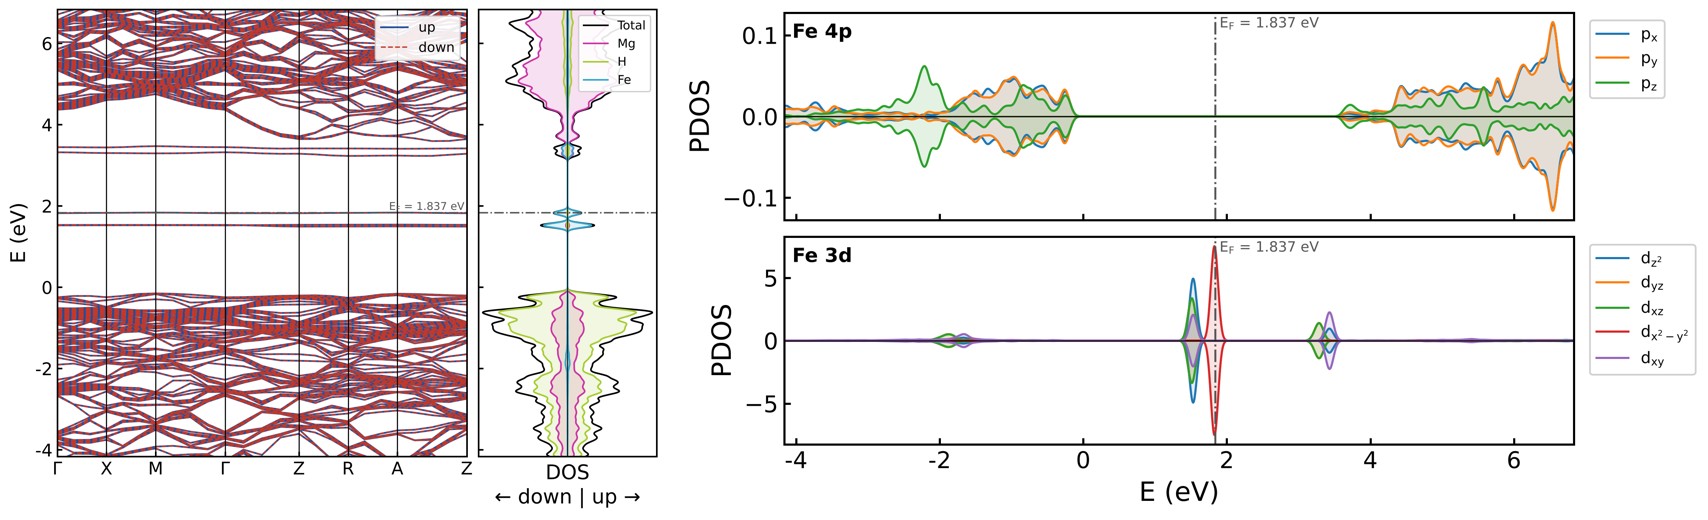
\includegraphics[width=\linewidth]{fermi_python.png}
\caption{MgH$_2$:Fe calculado com o CASTEP e analisado pelo BrUMaRe: bandas com DOS total e projetada (esquerda) e PDOS 4p/3d do Fe (direita), na escala original de energia, com o nível de Fermi marcado.}\label{fig:mgh2}
\end{figure}

\section{Limitações e trabalhos futuros}

O gap e as bordas são avaliados nos pontos $\mathbf k$ do caminho calculado; a DOS obtida de um caminho é apenas ilustrativa. A correção do gap por tesoura não altera a dispersão das bandas nem a posição de níveis de defeito, para as quais são necessários funcionais híbridos ou DFT+U. As energias termodinâmicas não incluem energia de ponto zero. O refinamento das fronteiras de Bader está disponível apenas na linha de comando. Como trabalhos futuros, prevêem-se a função trabalho a partir do potencial eletrostático, as populações de orbitais cristalinos (COHP), dispersões de fônons, propriedades ópticas e o desdobramento de bandas.

\section{Considerações do capítulo}

O BrUMaRe reúne, num programa livre, análises que normalmente exigem várias ferramentas, para cinco programas de estrutura eletrônica, com resultados idênticos no navegador, no aplicativo e na linha de comando. A preservação do nível de Fermi, a exportação de dados em texto, a citação automática e a validação sistemática contra ferramentas consolidadas tornam as análises desta dissertação reprodutíveis e verificáveis. O programa, o tutorial em seis idiomas e a documentação teórica estão disponíveis publicamente.
